\subsubsection{Subtree Mutation}
\label{sec:keen:op:mut:subtree}
    One key technique among mutation operators in GP is the Subtree Mutation. It serves to adjust the genetic structure 
    of program trees.

    \begin{definition}[Subtree Mutation]
        The \textit{subtree mutation} operator works by selecting a node from a program tree. It then replaces the 
        subtree originating from this node with a new subtree. This process keeps the general shape of the program while 
        introducing fresh genetic elements, which might enhance the program's effectiveness.

        To paint a mathematical portrait of this operation:

        \begin{equation}
        M_{subtree}: \mathbb{P} \times [0,\, 1] \times [0,\, 1] \times [0,\, 1] \rightarrow \mathbb{P};\;
        (P,\, \mu_\textbf{i},\, \mu_\textbf{c},\, \mu_\textbf{g}) 
            \mapsto M_{subtree}(P,\, \mu_\textbf{i},\, \mu_\textbf{c},\, \mu_\textbf{g})
        \end{equation}

        Breaking down the parameters:

        \begin{itemize}
        \item \(P\): Embodies a population of program trees.
        \item \(\mu_\textbf{i}\): Denotes the probability of an individual experiencing mutation.
        \item \(\mu_\textbf{c}\): Signifies the likelihood of a chromosome's selection for mutation.
        \item \(\mu_\textbf{g}\): Represents the probability of a gene's selection for mutation.
        \end{itemize}
    \end{definition}

    In the \textit{Keen} framework, the Subtree Mutation process happens like this:

    \begin{code}{
        Explaining Subtree Mutation in \textit{Keen}
    }{label=lst:keen:op:mut:subtree}{kotlin}
        val targetNode = choose random node from program tree
        val newSubtree = create a new subtree
        val mutatedTree = replace targetNode's subtree in program tree with newSubtree
    \end{code}

    In essence, the Subtree Mutation in \textit{Keen} adds new genetic components without heavily changing the main 
    structure of the tree.

    \begin{remark}
        The Subtree Mutation is great at making significant genetic changes. However, it's important to make sure the 
        new subtrees fit well with the problem you're solving. Without this check, you might end up with trees that 
        don't make sense or are too complex.

        \textit{Keen} handles this by using generation methods mentioned in \vref{sec:keen:gp:primitives:gen}.
    \end{remark}

    The beauty of the Subtree Mutation method lies in its balance. It keeps what works while trying out new genetic 
    possibilities.

    For a visual representation of the Subtree Mutation process, see \vref{fig:keen:op:mut:subtree}.

    \begin{figure}[ht!]
        \centering
        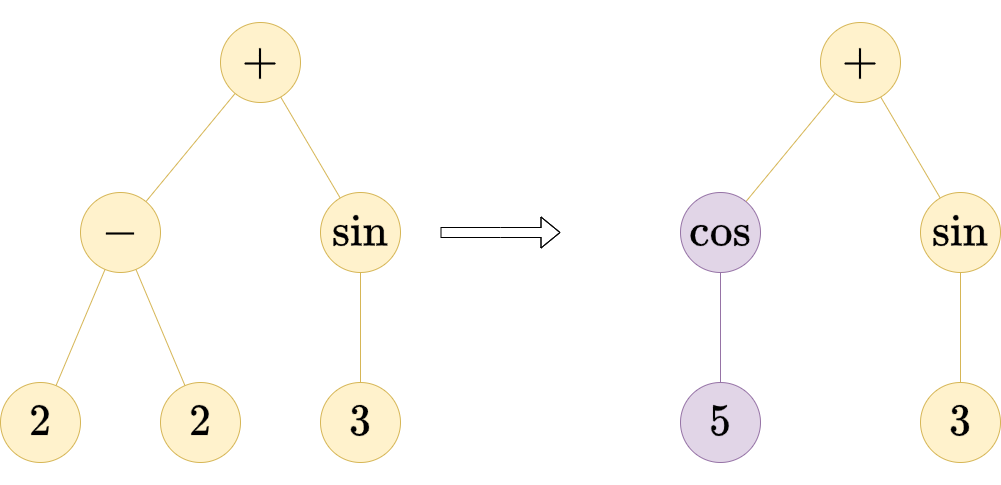
\includegraphics[width=0.5\textwidth]{img/keen/STM.png}
        \caption{
            A visual guide to the Subtree Mutation process. The operator picks a node and replaces its attached subtree 
            with a new one, giving a changed but still recognizable program tree.
        }
        \label{fig:keen:op:mut:subtree}
    \end{figure}
